%%
%% presentation.tex
%%
%% Made by Jakub Kuźma
%% Login   <kuba@jah.pl>
%%
%% Started on  Fri Oct 24 19:44:04 2008 Jakub Kuźma
%% Last update Fri Oct 24 19:44:04 2008 Jakub Kuźma
%%

\documentclass[12t]{beamer}
\usepackage[utf8]{inputenc}
\usepackage[T2A]{fontenc}
\usepackage[polish]{babel}
\usepackage{polski}
\usepackage{graphicx}
\usepackage{color}
\input{pygments}

\usetheme{Pittsburgh}

\author{Silesian Ruby Users' Group}
\title{Ruby on Rails}
\setbeamercovered{transparent}
%\setbeameroption{show notes}

\begin{document}

\frame{\titlepage}

\section{Wstęp}
\begin{frame}
  \frametitle{Dlaczego web development?}
  \begin{itemize}
  \item przenośność
  \item niezależność od systemów operacyjnych i przeglądarek
  \item łatwe zarządzanie i utrzymanie
  \end{itemize}
\end{frame}

\begin{frame}
  \frametitle{Dlaczego Ruby on Rails?}
  \begin{itemize}
  \item przyjemność z programowania
  \item open source
  \item czytelność kodu
  \item propagowanie dobrych praktyk programistycznych
  \item szybkość programowania
  \item łatwość reagowania na zmiany
  \item niezależność od systemu operacyjnego
  \item niezależność od środowiska pracy (NetBeans, RadRails, Emacs,
    Vim, JEdit)
  \end{itemize}
\end{frame}

\section{Ruby}
\begin{frame}
  \frametitle{Ruby}
  \begin{itemize}
  \item 1995 rok, Yukihiro Matsumoto aka Matz
  \item inspirowany przez CLU, Eiffel, Lisp, Perl, Python, Smalltalk
  \item interpretowany
  \item wieloparadygmatowy
  \item bardzo wysokiego poziomu (VHLL)
  \end{itemize}
\end{frame}

\begin{frame}
  \frametitle{Ruby, c.d.}
  \begin{itemize}
  \item w pełni obiektowy
  \item prosta składnia, samokomentujący się kod
    \begin{block}{Przykłady}
      \begin{Verbatim}[commandchars=@\[\]]
@PYaW["]@PYaW[!dlroW ,olleH]@PYaW["]@PYbe[.]reverse

@PYag[3]@PYbe[.]times { @PYaX[puts] @PYaW["]@PYaW[Ruby rulez!]@PYaW["] }

@PYaX[exit] @PYay[if] restaurants@PYbe[.]include? @PYaW["]@PYaW[wiedeński]@PYaW["]

@PYay[raise] @PYaq[ArgumentError] @PYay[unless] argument@PYbe[.]kind_of? @PYaX[String]

@PYbe[@lb[]]@PYag[5],@PYag[20],@PYag[5],@PYag[10],@PYag[10],@PYag[30]@PYbe[@rb[]]@PYbe[.]sort@PYbe[.]last

@PYay[return] list@PYbe[.]uniq @PYay[if] list@PYbe[.]respond_to? @PYaW["]@PYaW[uniq]@PYaW["]
\end{Verbatim}

    \end{block}
  \end{itemize}
\end{frame}

\begin{frame}
  \frametitle{Nazewnictwo}
  \begin{small}
    \begin{Verbatim}[commandchars=@\[\]]
@PYar[$uczelnia] @PYbe[=] @PYaW["]@PYaW[Polibuda]@PYaW["]

@PYay[class] @PYaN[Straz]
  @PYay[def] @PYaN[self]@PYbe[.]@PYaK[wezwij](akademik)
    @PYaf[# ...]
  @PYay[end]
@PYay[end]

@PYay[class] @PYaN[OndraszekPortierka]
  @PYaq[AKADEMIK] @PYbe[=] @PYat[:ondraszek]
  @PYaG[@at[]@at[]klucze] @PYbe[=] @PYaq[OndraszekKlucze]@PYbe[.]new
  @PYay[def] @PYaK[initialize](kolor)
    @PYaR[@at[]kamizelka] @PYbe[=] @PYaq[Kamizelka]@PYbe[.]new(kolor)
  @PYay[end]
  @PYay[def] @PYaK[wezwij_straz]
    @PYaq[Straz]@PYbe[.]wezwij(@PYaq[AKADEMIK])
  @PYay[end]
@PYay[end]
\end{Verbatim}

  \end{small}
  \note{Styl formatowania kodu nie jest narzucony z góry, wcięcia nie
    mają dla interpretera żadnego znaczenia}
\end{frame}

\begin{frame}
  \frametitle{Stałe są zmienne}
  \begin{Verbatim}[commandchars=@\[\]]
@PYaq[SRUG_EMAIL] @PYbe[=] @PYaW["]@PYaW[spotkania@at[]srug.pl]@PYaW["]
@PYaq[SRUG_EMAIL] @PYbe[=] @PYaW["]@PYaW[admin@at[]srug.pl]@PYaW["]
@PYaf[# warning: already initialized constant SRUG_EMAIL]
\end{Verbatim}

\end{frame}

\begin{frame}
  \begin{itemize}
  \item omijane przez garbage collector
  \item wykorzystywane m.in. jako klucze w tablicach haszujących
  \end{itemize}
  \frametitle{Symbole}
  \begin{block}{Przykład}
    \begin{Verbatim}[commandchars=@\[\]]
@PYaW["]@PYaW[string]@PYaW["]@PYbe[.]object_id
@PYbe[-]@PYag[606377798]
@PYaW["]@PYaW[string]@PYaW["]@PYbe[.]object_id
@PYbe[-]@PYag[606384058]
@PYat[:symbol]@PYbe[.]object_id
@PYag[204898]
@PYat[:symbol]@PYbe[.]object_id
@PYag[204898]
\end{Verbatim}

  \end{block}
\end{frame}

\begin{frame}
  \frametitle{Duck typing}
  \begin{itemize}
  \item rozpoznawanie typów na podstawie ich zachowania, a nie deklaracji
  \end{itemize}
\end{frame}

\begin{frame}
  \begin{quote}
    “If it walks like a duck and quacks like a duck, I would call it a
    duck.”

    \hfill James Whitcomb Riley
  \end{quote}
\end{frame}

\begin{frame}
  \frametitle{Duck typing - przykład}
 \begin{small}
    \begin{Verbatim}[commandchars=@\[\]]
@PYay[class] @PYaN[Duck]
  @PYay[def] @PYaK[quack]
    @PYaW["]@PYaW[Quack!]@PYaW["]
  @PYay[end]
@PYay[end]
@PYay[class] @PYaN[Dog]
  @PYay[def] @PYaK[quack]
    @PYaW["]@PYaW[Quack!]@PYaW["]
  @PYay[end]
@PYay[end]
@PYay[def] @PYaK[make_it_quack](duck)
  @PYaX[puts] duck@PYbe[.]quack
@PYay[end]

duck @PYbe[=] @PYaq[Duck]@PYbe[.]new
dog @PYbe[=] @PYaq[Dog]@PYbe[.]new

make_it_quack(duck)
@PYaf[# Quack!]
make_it_quack(dog)
@PYaf[# Quack!]
\end{Verbatim}

  \end{small}
\end{frame}

\begin{frame}
  \frametitle{Domknięcia}
  \begin{itemize}
  \item bloki kodu mogą być przekazywane jako argumenty i zwracane
    jako wynik działania funkcji (metody)
  \item są podstawową cechą języków funkcyjnych
  \item odwołują się do zmiennych z kontekstu, w którym zostały
    stworzone, a nie z którego są wywoływane
  \end{itemize}
\end{frame}

\begin{frame}
  \frametitle{Domknięcia - przykład}
  \begin{Verbatim}[commandchars=@\[\]]
@PYay[def] @PYaK[say_something]
  something @PYbe[=] @PYaW["]@PYaW[Hello!]@PYaW["]
  @PYaX[lambda] { @PYaX[puts] something }
@PYay[end]

result @PYbe[=] say_something
something @PYbe[=] @PYaW["]@PYaW[Bye!]@PYaW["]
result@PYbe[.]call
@PYaf[# Hello!]
\end{Verbatim}

\end{frame}

\begin{frame}
  \frametitle{Domknięcia - wykorzystanie}
  \begin{Verbatim}[commandchars=@\[\]]
@PYag[3]@PYbe[.]times { @PYaX[print] @PYaW["]@PYaW[SRUG]@PYaW["] }
@PYaf[# SRUGSRUGSRUG]

@PYag[5]@PYbe[.]upto(@PYag[10]) { @PYbe[|]i@PYbe[|] @PYaX[print] i, @PYaW["]@PYaW[ ]@PYaW["] }
@PYaf[# 5 6 7 8 9 10]

@PYbe[@lb[]]@PYaW["]@PYaW[Żubr]@PYaW["], @PYaW["]@PYaW[Żywiec]@PYaW["], @PYaW["]@PYaW[Harnaś]@PYaW["]@PYbe[@rb[]]@PYbe[.]select @PYay[do] @PYbe[|]drink@PYbe[|]
  drink@PYbe[.]beer?
@PYay[end]
@PYaf[#=> @lb[]"Żubr", "Żywiec"@rb[]]

@PYaX[open] @PYaW["]@PYaW[data.txt]@PYaW["] @PYay[do] @PYbe[|]file@PYbe[|]
  file@PYbe[.]each_line @PYay[do] @PYbe[|]line@PYbe[|]
    @PYaq[MyParser]@PYbe[.]parse line
  @PYay[end]
@PYay[end]
\end{Verbatim}

\end{frame}

\begin{frame}
  \frametitle{Cechy}
  \begin{itemize}
  \item dziedziczenie jednobazowe
  \item moduły zapewniają rodzaj dziedziczenia wielobazowego
    pozwalający włączyć gotową implementację zbioru metod do danej
    klasy (\emph{mixin})
    \note[item]{Moduły pełnią też rolę przestrzeni nazw}
  \item dziedziczenia używa się znacznie oszczędniej i rzadziej niż
    np. w Javie
  \end{itemize}
\end{frame}

\begin{frame}
  \frametitle{Cechy, c.d.}
  \begin{itemize}
  \item bogata biblioteka standardowa
  \item garbage collector
  \item przeciążanie operatorów
  \item liczby całkowite o dowolnych rozmiarach
  \item wyrażenia regularne wbudowane w składnię
  \end{itemize}
\end{frame}

\subsection{Otwarte klasy}
\begin{frame}
  \frametitle{Otwarte klasy - przykład}
  \begin{Verbatim}[commandchars=@\[\]]
@PYay[class] @PYaN[Array]
  @PYay[def] @PYaK[shuffle]
    sort_by { @PYaX[rand] }
  @PYay[end]
  @PYay[def] @PYaK[shuffle!]
    @PYaX[self]@PYbe[.]replace shuffle
  @PYay[end]
@PYay[end]

a @PYbe[=] @PYbe[@lb[]]@PYag[1], @PYag[2], @PYag[3], @PYag[4], @PYag[5], @PYag[6], @PYag[7], @PYag[8], @PYag[9]@PYbe[@rb[]]
a@PYbe[.]shuffle!
@PYaf[#=> @lb[]2, 9, 4, 5, 1, 7, 8, 3, 6@rb[]]
\end{Verbatim}

  \note{Uzupełniamy klasę z biblioteki standardowej - używamy metody
    shuffle tak jakby była tam od zawsze.}
  \note{Ze względu na częste użycie metoda shuffle znalazła się w
    bibliotece standardowej w Ruby 1.8.7}
\end{frame}

\subsection{Monkey patching}
\begin{frame}
  \frametitle{Monkey patching - problem}
  \begin{Verbatim}[commandchars=@\[\]]
@PYay[class] @PYaN[Array]
  alias_method @PYat[:old_index], @PYat[:index]

  @PYay[def] @PYaK[index](obj @PYbe[=] @PYaj[nil])
    @PYay[if] obj@PYbe[.]nil?
      @PYaX[self]@PYbe[.]each_with_index @PYay[do] @PYbe[|]e, i@PYbe[|]
        @PYay[return] i @PYay[if] @PYay[yield] e
      @PYay[end]
      @PYaj[nil]
    @PYay[else]
      old_index(obj)
    @PYay[end]
  @PYay[end]
@PYay[end]
\end{Verbatim}

  \note{Fajnie byłoby, gdyby metoda index przyjmowała blok i zwróciła
    w tym przypadku index równy 6}
\end{frame}

\begin{frame}
  \frametitle{Monkey patching - rozwiązanie}
  \input{monkeypatching2}
  \note{Podobnie jak w poprzednim przypadku - metoda index przyjmuje
    blok w Ruby 1.8.7}
\end{frame}

\subsection{Metaprogramowanie}
\begin{frame}
  \frametitle{Metaprogramowanie}
  \begin{itemize}
  \item metaprogramowanie w Rubim jest \textbf{proste}
  \item dysponujemy programowalnym językiem programowania
  \item główne narzędzie służące do budowy tzw. DSL
  \end{itemize}
\end{frame}

\begin{frame}[fragile]
  \frametitle{Metaprogramowanie - przykład}
  \begin{Verbatim}[commandchars=@\[\]]
@PYay[class] @PYaN[Module]
  @PYay[def] @PYaK[my_attr_accessor](@PYbe[*]symbols)
    symbols@PYbe[.]each @PYay[do] @PYbe[|]symbol@PYbe[|]
      @PYaX[module_eval] @PYap[%{]@PYap[def ]@PYbf[#{]symbol@PYbf[}]
@PYap[                      @at[]]@PYbf[#{]symbol@PYbf[}]
@PYap[                    end]@PYap[}]
      @PYaX[module_eval] @PYap[%{]@PYap[def ]@PYbf[#{]symbol@PYbf[}]@PYap[=(value)]
@PYap[                      @at[]]@PYbf[#{]symbol@PYbf[}]@PYap[ = value]
@PYap[                    end]@PYap[}]
    @PYay[end]
  @PYay[end]
@PYay[end]
\end{Verbatim}

\end{frame}

\begin{frame}[fragile]
  \frametitle{Metaprogramowanie - przykład, c.d.}
  \begin{Verbatim}[commandchars=@\[\]]
@PYay[class] @PYaN[Song]
  @PYaj[attr_accessor] @PYat[:name], @PYat[:duration]
@PYay[end]

song @PYbe[=] @PYaq[Song]@PYbe[.]new
song@PYbe[.]name, song@PYbe[.]duration @PYbe[=] @PYaW["]@PYaW[Miles Davis - So What]@PYaW["], @PYag[565]
@PYaX[puts] @PYaW["]@PYbf[#{]song@PYbe[.]name@PYbf[}]@PYaW[, ]@PYbf[#{]song@PYbe[.]duration@PYbf[}]@PYaW[ s]@PYaW["]
\end{Verbatim}

  \note{To nie jest specjalna składnia - to zwykłe wywołanie metody
    zadeklarowanej w klasie Module}
\end{frame}

\begin{frame}[fragile]
  \frametitle{Metaprogramowanie - przykład, c.d.}
  \begin{Verbatim}[commandchars=@\[\]]
@PYay[class] @PYaN[Song]
  @PYay[def] @PYaK[name]
    @PYaR[@at[]name]
  @PYay[end]
  @PYay[def] @PYaK[name]@PYbe[=](value)
    @PYaR[@at[]name] @PYbe[=] value
  @PYay[end]
  @PYay[def] @PYaK[duration]
    @PYaR[@at[]duration]
  @PYay[end]
  @PYay[def] @PYaK[duration]@PYbe[=](value)
    @PYaR[@at[]duration] @PYbe[=] value
  @PYay[end]
@PYay[end]
\end{Verbatim}

  \note{Wiele osób w dalszym ciągu traci czas na pisanie getterów i
    setterów w np. Javie}
  \note{nie musimy pisać funkcji - attr_accessor, attr_reader,
    attr_writer są w bibliotece standardowej. Zostały napisane w C}
\end{frame}

\subsection{Użycie method\_missing}
\begin{frame}[fragile]
  \frametitle{Użycie method\_missing}
  \begin{Verbatim}[commandchars=@\[\]]
@PYay[class] @PYaN[SupermarketTeller]
  @PYay[def] @PYaK[method_missing](method_name, @PYbe[*]args)
    @PYay[if] method_name@PYbe[.]to_s@PYbe[.]include? @PYaW["]@PYaW[lidl]@PYaW["]
      @PYaX[puts] @PYaW["]@PYaW[Lidl jest tani!]@PYaW["]
    @PYay[else]
      @PYay[raise] @PYaq[NoMethodError],
        @PYaW["]@PYaW[undefined method `]@PYbf[#{]method_name@PYbf[}]@PYaW[' for ]@PYbf[#{]@PYaX[self]@PYbf[}]@PYaW["]
    @PYay[end]
  @PYay[end]
@PYay[end]
\end{Verbatim}

\end{frame}

\begin{frame}[fragile]
  \frametitle{Użycie method\_missing, c.d.}
  \begin{Verbatim}[commandchars=@\[\]]
supermarket_teller @PYbe[=] @PYaq[SupermarketTeller]@PYbe[.]new

supermarket_teller@PYbe[.]jaki_jest_lidl?
@PYaf[# Lidl jest tani!]

supermarket_teller@PYbe[.]jaka_jest_biedronka?
@PYaf[# NoMethodError: undefined method ...]
\end{Verbatim}

  \note{Dla zaoszczędzenia czasu nie będziemy prezentować jak osiągnąć
    ten efekt w tradycyjny sposób}
\end{frame}

\begin{frame}
  \frametitle{Podsumowanie}
  \begin{itemize}
  \item „pseudo-code that runs” - skupianie się na rozwiązaniu
    problemu, nie na języku
  \item język zaprojektowany \textbf{dla ludzi}
  \item radość z programowania
  \item TIMTOWTDI - wolność wyboru (jak w Perlu, przeciwnie niż w
    Pythonie)
  \item zasada najmniejszego zaskoczenia - Ruby jest intuicyjny
  \end{itemize}
  \note{Stworzony by cieszyć}
\end{frame}

\section{Ruby - dodatki}
\begin{frame}
  \frametitle{RubyGems}
  system paczek: gem install rails
\end{frame}

\begin{frame}
  \frametitle{Rake}
  \begin{itemize}
  \item Rake - Ruby Make
  \item przykłady
  \end{itemize}
\end{frame}

\begin{frame}
  \frametitle{RSpec}
  \begin{itemize}
  \item framework BDD
  \item przykłady
  \end{itemize}
\end{frame}

\section{Ruby - rozwój}
\begin{frame}
  \frametitle{Ruby - rozwój}
  \begin{itemize}
  \item implementacje: MRI, Ruby Enterprise, JRuby, IronRuby
  \item maszyny wirtualne: MagLev, Rubinius, YARV
  \item Github
  \end{itemize}
\end{frame}

\section{Ruby on Rails}
\begin{frame}
  \frametitle{Ruby on Rails}
  \begin{itemize}
  \item David Heinemeier Hansson, 2004 r.
  \item kompletny framework do tworzenia aplikacji internetowych
    opartych o bazy danych
  \item wzorzec MVC
  \end{itemize}
\end{frame}

\begin{frame}
  \frametitle{Rails way}
  \begin{itemize}
  \item Convention over Configuration
  \item Don't Repeat Yourself
  \end{itemize}
\end{frame}

\begin{frame}
  \frametitle{Z czego składa się Rails?}
  \begin{itemize}
  \item ActiveRecord
  \item ActionPack
  \item ActiveResource
  \item ActionMailer
  \item ActiveSupport
  \end{itemize}
\end{frame}

\begin{frame}
  \frametitle{Architektura Rails}
  \begin{figure}
    \centering
    \includegraphics[width=\linewidth]{railsarchitecture.png}
  \end{figure}
\end{frame}

\begin{frame}[fragile]
  \frametitle{Zaczynamy!}
  \begin{columns}[T]
    \begin{column}{2.3cm}
      \includegraphics[width=2.3cm]{structure.png}
    \end{column}
    \begin{column}{7.5cm}
\begin{verbatim}
# gem install rails

$ rails myapp

$ cd myapp

$ ./script/server
\end{verbatim}
    \end{column}
  \end{columns}
\end{frame}

\begin{frame}
  \frametitle{ActiveRecord}
  \begin{itemize}
  \item domyślny ORM dla Rails
  \item są też inne opcje (np. DataMapper)
  \item implementacja wzorca Active Record
  \end{itemize}
\end{frame}

\begin{frame}
  \begin{quote}
    “I have never seen an Active Record implementation as complete or as useful as Rails”

    \hfill Martin Fowler
  \end{quote}
  \note{M.Fowler jest autorem książek i znanym wykładowcą z tematyki
    architektury oprogramowania, specjalizującym się w analizie
    obiektowej i projektowaniu, UML, wzorcach projektowych, metodykach
    zwinnych, w tym Programowania ekstremalnego}
\end{frame}

\begin{frame}
  \frametitle{ActiveRecord - co dostajemy?}
  \begin{itemize}
  \item prosta konfiguracja
  \item migracje bazy danych
  \item proste tworzenie asocjacji
  \item zapytania
  \item walidatory
  \item wywołania zwrotne
  \item transakcje
  \item kilka innych rzeczy
  \end{itemize}
\end{frame}

% WYRZUCIĆ, CZY NIE WYRZUCIĆ? Oto jest pytanie!
\begin{frame}
  \frametitle{ActiveRecord - konfiguracja}
  \begin{itemize}
  \item nie wymaga konfiguracji za pomocą setek linii XML-a
  \item mapowanie tabel na modele - konwencja nad konfiguracją
  \end{itemize}
\end{frame}

\begin{frame}[fragile]
  \frametitle{ActiveRecord - szybki start}
\begin{verbatim}
development:
  adapter: mysql
  database: demo
  username: admin
  password: password
  host: localhost
\end{verbatim}
\begin{verbatim}
$ ./script/generate model post title:string content:text

$ rake db:migrate
\end{verbatim}
  \begin{Verbatim}[commandchars=@\[\]]
@PYay[class] @PYaN[Post] @PYbe[<] @PYaq[ActiveRecord]@PYbe[::]@PYaq[Base]
@PYay[end]

@PYaq[Post]@PYbe[.]create @PYat[:title] @PYbe[=]@PYbe[>] @PYaW["]@PYaW[SRUG]@PYaW["],
            @PYat[:content] @PYbe[=]@PYbe[>] @PYaW["]@PYaW[Ruby on Rails]@PYaW["]
\end{Verbatim}

\end{frame}

\begin{frame}
  \frametitle{ActiveRecord - migracje}
  \begin{itemize}
  \item proste w użyciu wersjonowanie schematu bazy, historia zmian
  \item Ruby zamiast SQL-a
    \note{Uzyskujemy przenośność pomiędzy różnymi silnikami
      bazodanowymi}
  \item praca w zespołach
  \end{itemize}
\end{frame}

\begin{frame}[fragile]
  \frametitle{ActiveRecord - migracje - przykład}
  \begin{Verbatim}[commandchars=@\[\]]
@PYay[class] @PYaN[CreateStudents] @PYbe[<] @PYaq[ActiveRecord]@PYbe[::]@PYaq[Migration]
  @PYay[def] @PYaN[self]@PYbe[.]@PYaK[up]
    create_table @PYat[:students] @PYay[do] @PYbe[|]t@PYbe[|]
      t@PYbe[.]string @PYat[:name]
      t@PYbe[.]integer @PYat[:beers_count], @PYat[:null] @PYbe[=]@PYbe[>] @PYaj[false]
      t@PYbe[.]belongs_to @PYat[:dormitory]
      t@PYbe[.]timestamps
    @PYay[end]
  @PYay[end]

  @PYay[def] @PYaN[self]@PYbe[.]@PYaK[down]
    drop_table @PYat[:students]
  @PYay[end]
@PYay[end]
\end{Verbatim}

\end{frame}

\begin{frame}
  \frametitle{ActiveRecord - asocjacje}
  \begin{itemize}
  \item mapowanie powiązań pomiędzy obiektami ActiveRecord
  \item wyrażają relację takie jak “user has many projects” czy
    “product belongs to category”
  \item oparte na metaprogramowaniu
  \end{itemize}
\end{frame}

\begin{frame}[fragile]
  \frametitle{ActiveRecord - asocjacje - przykład}
  \begin{Verbatim}[commandchars=@\[\]]
@PYay[class] @PYaN[Post] @PYbe[<] @PYaq[ActiveRecord]@PYbe[::]@PYaq[Base]
  belongs_to @PYat[:category]
  has_many @PYat[:comments]
@PYay[end]

@PYay[class] @PYaN[Category] @PYbe[<] @PYaq[ActiveRecord]@PYbe[::]@PYaq[Base]
  has_many @PYat[:posts]
@PYay[end]

@PYay[class] @PYaN[Comment] @PYbe[<] @PYaq[ActiveRecord]@PYbe[::]@PYaq[Base]
  belongs_to @PYat[:post]
@PYay[end]
\end{Verbatim}

\end{frame}

\begin{frame}[fragile]
  \frametitle{ActiveRecord - asocjacje - przykład, c.d.}
  \begin{Verbatim}[commandchars=@\[\]]
category @PYbe[=] @PYaq[Category]@PYbe[.]find_by_title @PYaW["]@PYaW[SRUG]@PYaW["]
post @PYbe[=] category@PYbe[.]posts@PYbe[.]first
post@PYbe[.]comments@PYbe[.]find_all_by_author @PYaW["]@PYaW[John Doe]@PYaW["]
post@PYbe[.]comments@PYbe[.]create @PYat[:content] @PYbe[=]@PYbe[>] @PYaW["]@PYaW[useful comment]@PYaW["]
post@PYbe[.]comments@PYbe[.]last
post@PYbe[.]comments@PYbe[.]delete_all
\end{Verbatim}

\end{frame}

\begin{frame}
  \frametitle{ActiveRcord - zapytania}
  \begin{itemize}
  \item Różne sposoby budowania zapytań
  \item Nazwane zapytania
  \end{itemize}
\end{frame}

\begin{frame}[fragile]
  \frametitle{ActiveRecord - przykłady zapytań}
  \begin{footnotesize}
    \begin{Verbatim}[commandchars=@\[\]]
@PYaq[Movie]@PYbe[.]first
@PYaf[# SELECT * FROM "movies" LIMIT 1]

@PYaq[Book]@PYbe[.]last
@PYaf[# SELECT * FROM "books" ORDER BY books.id DESC LIMIT 1]

@PYaq[Beer]@PYbe[.]find(@PYag[1])
@PYaf[# SELECT * FROM "beers" WHERE ("beers"."id" = 1)]

@PYaq[Subject]@PYbe[.]find(@PYbe[@lb[]]@PYag[3], @PYag[5], @PYag[7]@PYbe[@rb[]])
@PYaf[# SELECT * FROM "subjects" WHERE ("subjects"."id" IN (3,5,7))]

@PYaq[Student]@PYbe[.]all(@PYat[:conditions] @PYbe[=]@PYbe[>] { @PYat[:beer_count] @PYbe[=]@PYbe[>] @PYag[10]@PYbe[.].@PYag[20] })
@PYaf[# SELECT * FROM "students" WHERE]
@PYaf[#  ("students"."beer_count" BETWEEN '10' AND '20')]
\end{Verbatim}

  \end{footnotesize}
\end{frame}

\begin{frame}[fragile]
  \frametitle{ActiveRecord - przykłady zapytań c.d.}
  \begin{footnotesize}
    \begin{Verbatim}[commandchars=@\[\]]
@PYaq[Post]@PYbe[.]all(@PYat[:conditions] @PYbe[=]@PYbe[>] @PYbe[@lb[]]@PYaW["]@PYaW[title LIKE ? ]@PYaW["], @PYaW["]@PYaW[Rails]@PYaW["]@PYbe[@rb[]])
@PYaf[# SELECT * FROM "posts" WHERE (title LIKE 'Rails')]

@PYaq[Post]@PYbe[.]first(@PYat[:include] @PYbe[=]@PYbe[>] @PYbe[@lb[]]@PYat[:category], @PYat[:comments]@PYbe[@rb[]])
@PYaf[# SELECT * FROM "posts" LIMIT 1]
@PYaf[# SELECT * FROM "categories" WHERE ("categories"."id" IN (1))]
@PYaf[# SELECT "comments".* FROM "comments" WHERE ("comments".post_id IN (1))]

@PYaq[User]@PYbe[.]first(@PYat[:conditions] @PYbe[=]@PYbe[>] { @PYat[:login] @PYbe[=]@PYbe[>] @PYaW["]@PYaW[srug]@PYaW["], @PYat[:password] @PYbe[=]@PYbe[>] @PYaW["]@PYaW[secret]@PYaW["] })
@PYaf[# SELECT * FROM "users" WHERE]
@PYaf[#   ("users"."password" = 'secret' AND "users"."login" = 'srug')]

@PYaq[User]@PYbe[.]first(@PYat[:conditions] @PYbe[=]@PYbe[>] { @PYat[:login] @PYbe[=]@PYbe[>] @PYbe[@lb[]]@PYaW["]@PYaW[srug]@PYaW["], @PYaW["]@PYaW[Srug]@PYaW["], @PYaW["]@PYaW[SRUG]@PYaW["]@PYbe[@rb[]]})
@PYaf[# SELECT * FROM "users" WHERE]
@PYaf[#   ("users"."login" IN ('srug','Srug','SRUG')) LIMIT 1]
\end{Verbatim}

  \end{footnotesize}
\end{frame}

\begin{frame}[fragile]
  \frametitle{ActiveRecord - przykłady zapytań c.d.}
  \begin{small}
    \begin{Verbatim}[commandchars=@\[\]]
@PYaq[Student]@PYbe[.]count
@PYaf[# SELECT count(*) AS count_all FROM "students"]

@PYaq[Product]@PYbe[.]sum(@PYat[:price])
@PYaf[# SELECT sum(price) AS sum_price FROM "products"]

@PYaq[Visit]@PYbe[.]average(@PYaW["]@PYaW[duration / 3600.0]@PYaW["], @PYat[:group_by] @PYbe[=]@PYbe[>] @PYaW["]@PYaW[day]@PYaW["])
@PYaf[# SELECT sum(duration / 3600.0)]
@PYaf[#   AS sum_duration_3600_0, day AS day]
@PYaf[#   FROM "visits" GROUP BY day]
\end{Verbatim}

  \end{small}
\end{frame}

\begin{frame}
  \frametitle{Named scope - przykłady}
  \begin{small}
    \begin{Verbatim}[commandchars=@\[\]]
@PYay[class] @PYaN[Post] @PYbe[<] @PYaq[ActiveRecord]@PYbe[::]@PYaq[Base]
  belongs_to @PYat[:category]

  named_scope @PYat[:recent], @PYaX[lambda] @PYay[do]
    { @PYat[:conditions] @PYbe[=]@PYbe[>] @PYbe[@lb[]]@PYaW["]@PYaW[created_at > ?]@PYaW["], @PYag[2]@PYbe[.]hours@PYbe[.]ago@PYbe[@rb[]] }
  @PYay[end]
  named_scope @PYat[:published],
              @PYat[:conditions] @PYbe[=]@PYbe[>] { @PYat[:published] @PYbe[=]@PYbe[>] @PYaj[true] }
@PYay[end]

@PYaq[Post]@PYbe[.]recent
@PYaf[# SELECT * FROM "posts"]
@PYaf[# WHERE (created_at > '2008-10-29 19:12:15')]

@PYaq[Post]@PYbe[.]recent@PYbe[.]published
@PYaf[# SELECT * FROM "posts"]
@PYaf[# WHERE (("posts"."published" = 't') AND]
@PYaf[#        (created_at > '2008-10-29 19:12:22'))]
\end{Verbatim}

  \end{small}
\end{frame}

\begin{frame}
  \frametitle{ActiveRecord - walidatory}
  \begin{itemize}
  \item gwarantują poprawność wprowadzanych danych
  \item przeniesienie walidacji z poziomu bazy danych do modelu
  \item można walidować: format, długość, obecność, unikalność,
    powiązane obiekty, etc.
  \item łatwe tworzenie własnych walidatorów
  \end{itemize}
\end{frame}

\begin{frame}
  \frametitle{ActiveRecord - walidatory - przykład}
  \begin{Verbatim}[commandchars=@\[\]]
@PYay[class] @PYaN[Post] @PYbe[<] @PYaq[ActiveRecord]@PYbe[::]@PYaq[Base]
  validates_presence_of     @PYat[:title],
                            @PYat[:content]
  validates_uniqueness_of   @PYat[:title],
                            @PYat[:scope] @PYbe[=]@PYbe[>] @PYat[:category_id]
  validates_format_of       @PYat[:title],
                            @PYat[:with] @PYbe[=]@PYbe[>] @PYak[/]@PYak[\]@PYak[A@lb[]]@PYak[\]@PYak[w]@PYak[\]@PYak[s@rb[]+]@PYak[\]@PYak[Z]@PYak[/]
  validates_numericality_of @PYat[:rating],
                            @PYat[:greater_than] @PYbe[=]@PYbe[>] @PYag[0]
  validate                  @PYat[:niceness_of_title]

  @PYay[def] @PYaK[niceness_of_title]
    errors@PYbe[.]add @PYat[:title], @PYaW["]@PYaW[is lousy]@PYaW["] @PYay[unless] title@PYbe[.]nice?
  @PYay[end]
@PYay[end]
\end{Verbatim}

\end{frame}

\begin{frame}
  \frametitle{ActiveRecord - wywołania zwrotne}
  \begin{itemize}
  \item wyzwalanie logiki przed lub po zmianie stanu obiektu
  \item manipulacja atrybutami obiektu przed jego utworzeniem,
    zapisem, usunięciem lub walidacją
  \item przeniesienie logiki z kontrolera do modelu
  \end{itemize}
\end{frame}

\begin{frame}
  \frametitle{ActiveRecord - callbacks - przykład}
  \begin{Verbatim}[commandchars=@\[\]]
@PYay[class] @PYaN[Post] @PYbe[<] @PYaq[ActiveRecord]@PYbe[::]@PYaq[Base]
  before_validation @PYat[:sanitize_title], @PYat[:escape_content]
  after_destroy @PYat[:clear_category_cache]

  @PYay[def] @PYaK[sanitize_title]
    title@PYbe[.]sanitize!
  @PYay[end]
  @PYaf[# ...]
@PYay[end]
\end{Verbatim}

\end{frame}

\begin{frame}
  \frametitle{ActiveRecord - transakcje}
  \begin{itemize}
  \item bloki kodu, w których gwarantowana jest atomowość wszystkich
    operacji na bazie danych
  \item różne modele w jednej transakcji
  \end{itemize}
  \begin{block}{Przykład}
    \begin{Verbatim}[commandchars=@\[\]]
transaction @PYay[do]
  david@PYbe[.]withdrawal @PYag[100]
  mary@PYbe[.]deposit @PYag[100]
@PYay[end]
\end{Verbatim}

  \end{block}
\end{frame}

% TODO może wywalić trzeba go
\begin{frame}
  \frametitle{ActiveRecord}
  \begin{itemize}
  \item Single Table Inheritance
  \item asocjacje polimorficzne
  \item optimistic locking
  \item acts\_as: state\_machine, taggable, nested\_set, commentable,
    dictionary, geocodable
  \end{itemize}
\end{frame}

\begin{frame}
  \frametitle{ActionPack}
  \begin{itemize}
  \item podział odpowiedzi aplikacji na dwie części:
    \begin{itemize}
    \item ActionController
    \item ActionView
    \end{itemize}
  \end{itemize}
\end{frame}

\begin{frame}
  \frametitle{ActionPack::ActionController}
  \begin{itemize}
  \item request zostaje skierowany do odpowiedniej akcji (routing)
  \item akcja zwraca odpowiedź do przeglądarki
    \begin{itemize}
    \item wyrenderowany widok
    \item przekierowanie
    \item błąd
    \end{itemize}
  \item cookies
  \item sesje
  \item flash
  \item filtry
  \end{itemize}
\end{frame}

\begin{frame}
  \frametitle{ActionPack::ActionController}
  \begin{small}
  \begin{Verbatim}[commandchars=@\[\]]
@PYay[class] @PYaN[BeersController] @PYbe[<] @PYaq[ApplicationController]
  @PYay[def] @PYaK[index]
    @PYaR[@at[]beers]@PYbe[=] @PYaq[Beer]@PYbe[.]all
  @PYay[end]
@PYay[end]
\end{Verbatim}

  \end{small}
\end{frame}

\begin{frame}
  \frametitle{ActionController::Routing}
  \begin{itemize}
  \item wiązanie URI z akcjami odpowiednich kontrolerów
  \item zasoby (REST)
  \item ścieżki nazwane
  \end{itemize}
  \begin{block}{Przykład}
    \begin{Verbatim}[commandchars=@\[\]]
@PYaq[ActionController]@PYbe[::]@PYaq[Routing]@PYbe[::]@PYaq[Routes]@PYbe[.]draw @PYay[do] @PYbe[|]map@PYbe[|]
  map@PYbe[.]resources @PYat[:beers]
@PYay[end]
\end{Verbatim}

  \end{block}
\end{frame}

\begin{frame}
  \frametitle{ActionController::Routing, przykłady}
  \begin{scriptsize}
    \begin{Verbatim}[commandchars=@\[\]]
@PYay[class] @PYaN[CategoriesController] @PYbe[<] @PYaq[ApplicationController]
  @PYaf[# GET /categories]
  @PYay[def] @PYaK[index]
  @PYay[end]
  @PYaf[# GET /categories/1]
  @PYay[def] @PYaK[show]
  @PYay[end]
  @PYaf[# GET /categories/new]
  @PYay[def] @PYaK[new]
  @PYay[end]
  @PYaf[# GET /categories/1/edit]
  @PYay[def] @PYaK[edit]
  @PYay[end]
  @PYaf[# POST /categories]
  @PYay[def] @PYaK[create]
  @PYay[end]
  @PYaf[# PUT /categories/1]
  @PYay[def] @PYaK[update]
  @PYay[end]
  @PYaf[# DELETE /categories/1]
  @PYay[def] @PYaK[destroy]
  @PYay[end]
@PYay[end]
\end{Verbatim}

  \end{scriptsize}
\end{frame}


\begin{frame}
  \frametitle{ActionPack::ActionView}
  \begin{itemize}
  \item szablony w widokach: ERb, Haml, Liquid i inne
  \item partiale
  \item helpery
  \end{itemize}
\end{frame}

\begin{frame}[fragile]
  \frametitle{ActionPack::ActionView - ERb}
  \begin{Verbatim}[commandchars=@\[\]]
@PYaZ[<table] @PYaP[class=]@PYad['beers'] @PYaP[id=]@PYad['important']@PYaZ[>]
  @PYaZ[<tr] @PYaP[class=]@PYad['header']@PYaZ[>]
    @PYaZ[<th]@PYaZ[>]Name@PYaZ[</th>]
    @PYaZ[<th]@PYaZ[>]Type@PYaZ[</th>]
  @PYaM[<%-] @PYaR[@at[]beers]@PYbe[.]each @PYay[do] @PYbe[|]beer@PYbe[|] @PYaM[%>]
  @PYaZ[<tr]@PYaZ[>]
    @PYaZ[<td]@PYaZ[>]@PYaM[<%=] beer@PYbe[.]name @PYaM[%>]@PYaZ[</td>]
    @PYaZ[<td]@PYaZ[>]@PYaM[<%=] beer@PYbe[.]type @PYaM[%>]@PYaZ[</td>]
  @PYaZ[</tr>]
  @PYaM[<%-] @PYay[end] @PYaM[%>]
@PYaZ[</table>]
\end{Verbatim}

\end{frame}

\begin{frame}[fragile]
  \frametitle{ActionPack::ActionView - HAML}
  \begin{footnotesize}
  \begin{columns}[T]
    \begin{column}{4cm}
      \begin{verbatim}
%table#beers.important
  %tr.header
    %th Name
    %th Type
  - @beers.each do |beer|
    %tr
      %td= beer.name
      %td= beer.type
\end{verbatim}

    \end{column}
    \begin{column}{6cm}
      \begin{Verbatim}[commandchars=@\[\]]
@PYaZ[<table] @PYaP[class=]@PYad['important'] @PYaP[id=]@PYad['beers']@PYaZ[>]
  @PYaZ[<tr] @PYaP[class=]@PYad['header']@PYaZ[>]
    @PYaZ[<th]@PYaZ[>]Name@PYaZ[</th>]
    @PYaZ[<th]@PYaZ[>]Type@PYaZ[</th>]
  @PYaZ[</tr>]
  @PYaZ[<tr]@PYaZ[>]
    @PYaZ[<td]@PYaZ[>]Pilsner Urquell@PYaZ[</td>]
    @PYaZ[<td]@PYaZ[>]pilsner@PYaZ[</td>]
  @PYaZ[</tr>]
  @PYaZ[<tr]@PYaZ[>]
    @PYaZ[<td]@PYaZ[>]Żywiec Porter@PYaZ[</td>]
    @PYaZ[<td]@PYaZ[>]porter@PYaZ[</td>]
  @PYaZ[</tr>]
@PYaZ[</table>]
\end{Verbatim}

    \end{column}
  \end{columns}
  \end{footnotesize}
\end{frame}

\begin{frame}
  \frametitle{ActiveSupport}
  \begin{Verbatim}[commandchars=@\[\]]
@PYag[40]@PYbe[.]minutes@PYbe[.]ago
@PYaf[#=> 2008-10-27 20:29:37 +0100]
@PYag[20]@PYbe[.]weeks@PYbe[.]from_now
@PYaf[#=> 2009-03-16 21:10:45 +0100]
@PYaq[Time]@PYbe[.]now@PYbe[.]at_beginning_of_year
@PYaf[#=> Tue Jan 01 00:00:00 +0100 2008]
@PYag[5]@PYbe[.]gigabytes
@PYaf[#=> 5368709120]
@PYaW["]@PYaW[good beer]@PYaW["]@PYbe[.]titleize@PYbe[.]pluralize
@PYaf[#=> "Good Beers"]
@PYbe[@lb[]]@PYaW["]@PYaW[Pilsner Urquell]@PYaW["], @PYaW["]@PYaW[Оболонь]@PYaW["], @PYaW["]@PYaW[Paulaner]@PYaW["]@PYbe[@rb[]]@PYbe[.]to_sentence
@PYaf[#=> "Pilsner Urquell, Оболонь and Paulaner"]
\end{Verbatim}

\end{frame}

\begin{frame}
  \frametitle{Serwery HTTP}
  \begin{itemize}
  \item Webrick
  \item Mongrel, Thin, Ebb
  \item Passenger (Apache 2)
  \end{itemize}
\end{frame}

\begin{frame}
  Przykłady wdrożeń
\end{frame}

\section{Ruby - podsumowanie}
\begin{frame}
  \frametitle{Jak zacząć}
  \begin{itemize}
  \item instant-rails
  \item github
  \item opensourcerails.com
  \item heroku.com
  \end{itemize}
\end{frame}

\begin{frame}
  \frametitle{Po 3 latach z Ruby - co się zmienia}
  \begin{itemize}
  \item Ruby jako pierwszy pozwolił mi czerpać radość z
    programowania. Wcześniej były Java, w C/C++ i inne
  \item Pragmatyzm. Prosty, czytelny kod. Mało kodu. Brak
    komentarzy. Więcej czasu na życie.
  \item Nie wrócę do już do języków ze statycznym typowaniem. Czytałem
    Bruca Eckela kiedy mówił, że statyczne typowanie to przyszłość. Po
    latach zmienił zdanie. To samo dotyczy deklarowania wyrzucanych
    wyjątków (patrz Java).
  \item Większy dystans i szersze spojrzenie na rzemiosło programowania.
  \item 1 nowy język programowania co roku (ObjC, Erlang, Lisp, ...)
  \end{itemize}
\end{frame}

\end{document}
